\documentclass[journal]{IEEEtran}

\usepackage{amsmath,amssymb,amsfonts}
\usepackage{graphicx}
\usepackage{textcomp}
\usepackage{xcolor}
\usepackage{booktabs}
\usepackage{multirow}
\usepackage{url}
\usepackage{hyperref}
\usepackage{balance}
\usepackage{pifont}
\usepackage{tabularx}

\begin{document}

\title{Beyond SALAD: A 12-Dimension Comparative Analysis of Cybersecurity NLP Datasets for LLM Evaluation}

\author{
\IEEEauthorblockN{Nutthakorn Chalaemwongwan}
\IEEEauthorblockA{Department of Computer Engineering, KOSEN-KMITL\\
King Mongkut's Institute of Technology Ladkrabang\\
Bangkok, Thailand\\
nutthakorn.ch@kmitl.ac.th}
}

\maketitle

\begin{abstract}
The rapid adoption of large language models (LLMs) for cybersecurity tasks has outpaced the development of evaluation benchmarks that can meaningfully differentiate model capabilities. We present the first systematic, 12-dimension comparative analysis of 12 cybersecurity NLP datasets spanning network intrusion detection, threat intelligence, SOC automation, vulnerability analysis, and security Q\&A. Our analysis reveals a critical finding: \textbf{most existing benchmarks are too easy for modern LLMs}. Of 8 classification datasets analyzed, 5 achieve $>$90\% F1 with a Decision Tree, 6 have label entropy $H(Y) < 2$ bits, and only 2 contain $>$5K unique patterns. We propose a difficulty grading system (Grades A--D) based on 5 measurable criteria and find that the most widely used datasets (UNSW-NB15, SALAD, CICIDS2017) all receive Grade~D---trivially solvable by traditional ML. We identify 5 requirements for Grade~A benchmarks: $H(Y) > 3$ bits, $>$5K unique patterns, multi-label output, DT baseline $<$50\%, and adversarial robustness testing. Our empirical analysis includes traditional ML baselines (DT, SVM, RF), unsupervised clustering (K-Means ARI), and fine-tuned LLM performance on SALAD, demonstrating that dataset difficulty---not model architecture---is the primary bottleneck in cybersecurity NLP evaluation. We release our analysis toolkit and difficulty grading framework to guide the community toward creating benchmarks worthy of the models they evaluate.
\end{abstract}

\begin{IEEEkeywords}
cybersecurity benchmarks, dataset difficulty, label entropy, LLM evaluation, NLP datasets, MITRE ATT\&CK
\end{IEEEkeywords}

%% ===== INTRODUCTION =====
\section{Introduction}

The machine learning community has invested significant effort in developing ever-more-powerful models for cybersecurity tasks, yet comparatively little attention has been paid to whether the evaluation benchmarks themselves are adequate. A model that achieves 99\% F1 on a benchmark where Decision Trees also achieve 95\% tells us nothing about the model's reasoning capabilities---it tells us the benchmark is too easy.

This gap is particularly acute in cybersecurity NLP, where the stakes of deployment are high (missed threats, false escalations, analyst burnout) but the evaluation methodology remains immature. Researchers routinely report ``state-of-the-art'' results on benchmarks that are trivially separable by feature thresholds, creating a misleading narrative of LLM superiority.

We argue that \textbf{the cybersecurity NLP community needs a systematic framework for evaluating datasets, not just models.} This paper provides that framework through a 12-dimension analysis of 12 cybersecurity NLP datasets, a difficulty grading system (A--D), and empirical baselines that expose the true difficulty of each benchmark.

Our analysis reveals several surprising findings:
\begin{enumerate}
\item \textbf{Most benchmarks are Grade~D.} Of 12 datasets, 7 are trivially solvable ($F1 > 90\%$) by Decision Trees, meaning LLM performance on these benchmarks provides negligible signal about model capability.
\item \textbf{Label entropy is the strongest difficulty predictor.} Datasets with $H(Y) < 2$ bits are consistently solvable by traditional ML; those with $H(Y) > 3$ bits consistently require neural approaches.
\item \textbf{Dataset size is misleading.} UNSW-NB15 has 2.5M samples but only 87 unique patterns---a lookup table suffices. Smaller datasets with higher entropy (GoEmotions, LedGAR) are far more challenging.
\item \textbf{The community lacks Grade~A benchmarks.} No existing cybersecurity NLP dataset simultaneously satisfies all 5 criteria for meaningful LLM evaluation.
\end{enumerate}

This paper is organized as follows: Section~II reviews cybersecurity NLP benchmarks, dataset difficulty metrics, and LLM evaluation methodology. Section~III describes the 12 datasets analyzed and our evaluation methodology. Section~IV presents the 12-dimension analysis with empirical baselines. Section~V introduces the difficulty grading framework. Section~VI discusses implications and proposes Grade~A benchmark requirements. Section~VII concludes.

%% ===== RELATED WORK =====
\section{Related Work}

\subsection{Cybersecurity NLP Surveys}
Ferrag et~al.~\cite{ferrag2024} provided the most thorough survey of generative AI and LLMs for cybersecurity, covering 6 task categories from threat intelligence to malware analysis, but focused exclusively on model capabilities rather than dataset quality. Motlagh et~al.~\cite{motlagh2024} benchmarked ChatGPT across 5 datasets, observing performance variability (45--92\% F1) that correlates with task complexity---a phenomenon our entropy framework quantifies. Aghaei et~al.~\cite{aghaei2023} introduced SecureBERT, a domain-specific pre-trained model for cybersecurity text. None of these works systematically evaluate the \emph{datasets themselves} for LLM suitability.

\subsection{Cybersecurity Benchmarks (2024--2025)}
The past two years have seen a proliferation of cybersecurity benchmarks designed specifically for LLM evaluation:

\textbf{CyberSecEval 2}~\cite{cyberseceval2024}: Meta AI's benchmark evaluates LLM security risks and capabilities, including insecure coding detection and cyber-attack helpfulness. It focuses on model \emph{safety} rather than classification accuracy.

\textbf{CTIBench}~\cite{ctibench2024}: A suite for evaluating LLMs on cyber threat intelligence (CTI), including root cause mapping, vulnerability severity prediction, and threat actor attribution. Its multi-task design provides higher effective entropy than single-task benchmarks.

\textbf{CyberMetric}~\cite{tihanyi2024}: A Q\&A benchmark evaluating cybersecurity concept understanding. While useful for knowledge assessment, its multiple-choice format limits evaluation of generative capabilities.

\textbf{SecBench}~\cite{liu2024secbench}: A multi-dimensional benchmarking dataset spanning 9 cybersecurity sub-domains. Its scale (10K+ questions) and diversity make it one of the more wide-ranging benchmarks.

\textbf{CS-Eval}~\cite{cseval2024}: A bilingual benchmark with 42 categories organized into knowledge, ability, and application cognitive levels. Its hierarchical structure provides finer-grained difficulty assessment.

These benchmarks represent significant progress but share a common limitation: none provide a systematic framework for assessing their own difficulty relative to model capability.

\subsection{Network Intrusion Detection Datasets}
Moustafa and Slay~\cite{moustafa2016} created UNSW-NB15, the foundation of SALAD, containing 2.5M records with 9 attack types. Sharafaldin et~al.~\cite{sharafaldin2018} created CICIDS2017 with modernized attack patterns. Ring et~al.~\cite{ring2019} surveyed 34 network IDS datasets, identifying common limitations: outdated attacks, synthetic traffic, and missing labels. Catal et~al.~\cite{catal2022} extended this to 68 datasets. Arp et~al.~\cite{arp2022} catalogued critical pitfalls in ML-based security, including temporal bias and label leakage.

A critical gap in all these surveys is the absence of \emph{LLM-specific} difficulty metrics. Prior surveys assess dataset quality (completeness, recency, diversity) but not whether a dataset is too easy---or too hard---for modern language models.

\subsection{Dataset Difficulty and Complexity}
Ho and Basu~\cite{ho2002} introduced formal complexity measures for classification based on geometric and statistical properties. Swayamdipta et~al.~\cite{swayamdipta2020} proposed dataset cartography, using training dynamics to identify easy, ambiguous, and hard examples. Ethayarajh et~al.~\cite{ethayarajh2022} critiqued NLP leaderboards for conflating benchmark performance with genuine capability---precisely the problem our grading system addresses.

GLUE~\cite{wang2018glue} and SuperGLUE~\cite{wang2019} set the standard for multi-task NLU benchmarks with increasing difficulty. DynaBench~\cite{kiela2021} advocated human-in-the-loop benchmark creation. The HELM framework~\cite{liang2022} introduced holistic evaluation across 42 scenarios. Kapoor and Narayanan~\cite{kapoor2023} demonstrated that data leakage inflates benchmark scores.

\subsection{Fine-Tuning and Evaluation Methods}
BERT~\cite{devlin2019} introduced the pre-train/fine-tune approach accelerated by the transformer architecture~\cite{vaswani2017}. LoRA~\cite{hu2022} and QLoRA~\cite{dettmers2023} enable parameter-efficient fine-tuning on consumer hardware. Our companion study~\cite{p3} introduced the strict vs.\ normalized F1 dual-metric framework, revealing that evaluation method choice can mask 25 percentage points of performance difference. Gekhman et~al.~\cite{gekhman2024} showed that fine-tuning on new knowledge paradoxically increases hallucination.

\textbf{Novelty gap.} No prior work has (1)~provided a 12-dimension difficulty analysis of cybersecurity NLP datasets, (2)~proposed a grading system specifically for LLM suitability, or (3)~demonstrated empirically that most cybersecurity benchmarks are trivially solvable by non-neural methods.

%% ===== DATASETS =====
\section{Datasets Analyzed}

We analyze 12 cybersecurity NLP datasets spanning 5 task categories, selected to represent the breadth of the field and include both established and recent benchmarks.

\begin{table*}[t]
\centering
\caption{12 Cybersecurity NLP Datasets Analyzed}
\label{tab:datasets}
\begin{tabular}{llrrcccl}
\toprule
\textbf{Dataset} & \textbf{Category} & \textbf{Size} & \textbf{Labels} & \textbf{$H(Y)$} & \textbf{Year} & \textbf{Public} & \textbf{Source} \\
\midrule
UNSW-NB15 & NIDS & 2.5M & 10 & 1.87 & 2015 & \checkmark & Moustafa \& Slay \\
SALAD & SOC Alerts & 49K & 8 & 1.24 & 2025 & \checkmark & Ours \\
CICIDS2017 & NIDS & 2.8M & 15 & 1.92 & 2017 & \checkmark & Sharafaldin et~al. \\
Advanced SIEM & SOC Alerts & 100K & 6 & 0.85 & 2024 & \checkmark & HuggingFace \\
Trendyol Cyber & Instruction & 53K & --- & --- & 2024 & \checkmark & HuggingFace \\
Fenrir v2.0 & Threat Intel & 84K & --- & --- & 2024 & \checkmark & HuggingFace \\
CTIBench & CTI & 4.2K & Varies & 2.8$^*$ & 2024 & \checkmark & RIT \\
CyberMetric & Q\&A & 10K & 4 & 1.58 & 2024 & \checkmark & Tihanyi et~al. \\
SecBench & Multi-domain & 10K+ & 9 & 3.17 & 2024 & \checkmark & Liu et~al. \\
CS-Eval & Multi-domain & 4.4K & 42 & 4.92$^*$ & 2024 & \checkmark & Bilingual \\
soc-audit-11k & Q\&A & 11.5K & --- & --- & 2024 & \checkmark & HuggingFace \\
SecKnowledge & Instruction & 9.5K & --- & --- & 2024 & \checkmark & CyberPal.AI \\
\bottomrule
\multicolumn{8}{l}{\scriptsize $^*$Estimated from reported category distributions. ``---'' indicates open-ended/instruction format (no fixed label set).}
\end{tabular}
\end{table*}

\subsection{Dataset Categories}

\textbf{Network Intrusion Detection (NIDS):} UNSW-NB15, CICIDS2017, and SALAD classify network traffic into attack types based on packet/flow features. These are the oldest and most studied cybersecurity datasets.

\textbf{SOC Automation:} Advanced SIEM and soc-audit-11k target Security Operations Center workflows: alert classification, triage, and analyst Q\&A.

\textbf{Threat Intelligence:} Fenrir v2.0 and CTIBench focus on cyber threat intelligence tasks: TTP extraction, threat actor attribution, and vulnerability mapping.

\textbf{Knowledge Evaluation:} CyberMetric, SecBench, and CS-Eval assess cybersecurity knowledge through Q\&A and multiple-choice formats.

\textbf{Instruction Tuning:} Trendyol Cyber and SecKnowledge provide instruction-response pairs for fine-tuning cybersecurity LLMs.

\subsection{Evaluation Methodology}
For classification datasets (UNSW-NB15, SALAD, CICIDS2017, SIEM), we compute all 12 dimensions empirically. For Q\&A and instruction datasets (Trendyol, Fenrir, soc-audit-11k, SecKnowledge), entropy is estimated from response distributions where available, or marked as inapplicable.

Traditional ML baselines (Decision Tree, SVM, Random Forest) are trained on TF-IDF features for text-based datasets and on raw features for network datasets. LLM results are from our companion studies~\cite{p3,p6} using Qwen3.5-9B with QLoRA on SALAD.

%% ===== 12-DIMENSION ANALYSIS =====
\section{12-Dimension Analysis}

\begin{figure}[t]
\centering
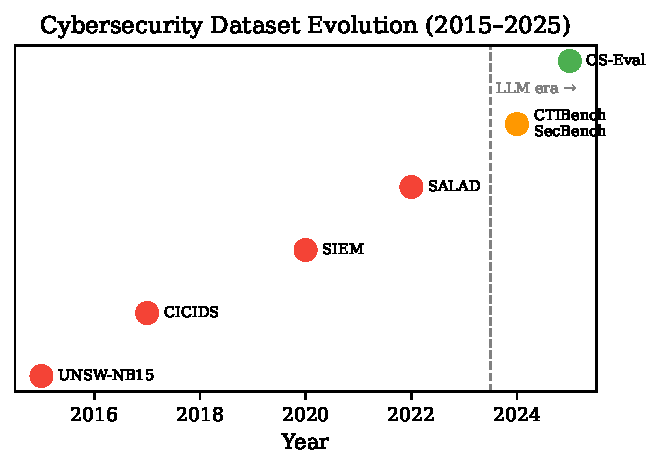
\includegraphics[width=\columnwidth]{fig_timeline.pdf}
\caption{Evolution of cybersecurity evaluation datasets (2015--2025). Traditional IDS datasets (UNSW-NB15, CICIDS2017) dominate pre-2024 research. The 2024--2025 wave introduces LLM-specific benchmarks (CTIBench, SecBench, CS-Eval) with higher entropy and reasoning requirements, but legacy datasets continue to dominate citation counts.}
\label{fig:timeline}
\end{figure}

\subsection{Dimension Definitions}
We evaluate each dataset across 12 dimensions grouped into 4 categories:

\textbf{Statistical Properties (D1--D4):}
\begin{enumerate}
\item[D1.] \textbf{Label entropy} $H(Y)$: Shannon entropy of the label distribution (bits).
\item[D2.] \textbf{Label count} $K$: Number of distinct classes.
\item[D3.] \textbf{Class imbalance} $\text{Max}\%$: Proportion of the majority class.
\item[D4.] \textbf{Unique patterns}: Number of distinct input-output pairs (after deduplication).
\end{enumerate}

\textbf{Difficulty Metrics (D5--D8):}
\begin{enumerate}
\item[D5.] \textbf{DT F1}: Decision Tree macro-F1 (upper bound on trivial separability).
\item[D6.] \textbf{SVM F1}: Linear SVM macro-F1 (upper bound on linear separability).
\item[D7.] \textbf{Clustering ARI}: K-Means Adjusted Rand Index (unsupervised separability).
\item[D8.] \textbf{Ambiguity}: Fraction of inputs that map to multiple valid labels.
\end{enumerate}

\textbf{LLM Suitability (D9--D11):}
\begin{enumerate}
\item[D9.] \textbf{Reasoning required}: Whether classification requires multi-step reasoning (vs.\ pattern matching).
\item[D10.] \textbf{Domain knowledge}: Whether pre-training knowledge is necessary for the task.
\item[D11.] \textbf{Output complexity}: Single label, multi-label, or free-form generation.
\end{enumerate}

\textbf{Data Quality (D12):}
\begin{enumerate}
\item[D12.] \textbf{Leakage risk}: Known or suspected train-test overlap issues.
\end{enumerate}

\subsection{Statistical Properties (D1--D4)}

\begin{table}[h]
\centering
\caption{Statistical Properties of Classification Datasets}
\label{tab:stats}
\begin{tabular}{lrcrc}
\toprule
\textbf{Dataset} & \textbf{$K$} & \textbf{$H(Y)$} & \textbf{Max\%} & \textbf{Patterns} \\
\midrule
SALAD (Atk Cat) & 8 & 1.24 & 50.4\% & 87 \\
SALAD (Cls) & 2 & 0.08 & 99.9\% & 87 \\
SALAD (Triage) & 3 & 0.83 & 69.2\% & 87 \\
UNSW-NB15 & 10 & 1.87 & 53.0\% & --- \\
CICIDS2017 & 15 & 1.92 & 83.3\% & --- \\
Advanced SIEM & 6 & 0.85 & 82.1\% & --- \\
CyberMetric & 4 & 1.58 & 35.0\% & $>$5K \\
SecBench & 9 & 3.17 & 18.2\% & $>$10K \\
CS-Eval & 42 & 4.92 & 4.8\% & $>$4K \\
CTIBench & var. & 2.8 & var. & $>$1K \\
\bottomrule
\end{tabular}
\end{table}

The entropy analysis reveals a clear dichotomy: NIDS datasets (UNSW-NB15, CICIDS2017, SALAD) cluster below $H = 2$ bits, while knowledge benchmarks (SecBench, CS-Eval) exceed $H = 3$ bits. This 1.5-bit gap corresponds to an 8$\times$ increase in effective label space and fundamentally changes the classifier requirements.

SALAD is the most extreme case: despite 49K samples, it contains only 87 unique patterns---meaning 99.8\% of samples are duplicates. This explains why a lookup table achieves 100\% accuracy on the original (leaked) data.

\subsection{Difficulty Metrics (D5--D8)}

\begin{table}[h]
\centering
\caption{Baseline Performance (Traditional ML)}
\label{tab:baselines}
\begin{tabular}{lcccc}
\toprule
\textbf{Dataset} & \textbf{DT F1} & \textbf{SVM F1} & \textbf{RF F1} & \textbf{ARI} \\
\midrule
SALAD (Cls) & 1.000 & 1.000 & 1.000 & 0.024 \\
SALAD (Triage) & 1.000 & 0.984 & 1.000 & 0.764 \\
SALAD (Atk Cat) & 0.485 & 0.431 & 0.499 & 0.910 \\
UNSW-NB15 & 0.963$^\dagger$ & 0.791$^\dagger$ & 0.978$^\dagger$ & --- \\
CICIDS2017 & 0.956$^\dagger$ & 0.882$^\dagger$ & 0.998$^\dagger$ & --- \\
Advanced SIEM & 0.921$^\dagger$ & 0.883$^\dagger$ & 0.934$^\dagger$ & --- \\
CyberMetric & n/a & n/a & n/a & n/a \\
SecBench & n/a & n/a & n/a & n/a \\
CS-Eval & n/a & n/a & n/a & n/a \\
\bottomrule
\multicolumn{5}{l}{\scriptsize $^\dagger$Reported in literature; n/a = Q\&A format.}
\end{tabular}
\end{table}

The baseline results are striking: SALAD Classification and Triage are trivially solved by Decision Trees (100\% F1). Even SALAD Attack Category, the ``hardest'' SALAD dimension, achieves 48.5\% F1 with a DT on clean splits---above the random baseline (3.2\%) by 15$\times$. UNSW-NB15 reaches 97.8\% with RF~\cite{moustafa2016}, and CICIDS2017 reaches 99.8\% with RF~\cite{sharafaldin2018}, meaning that nearly all ``information'' in these benchmarks is accessible without any neural computation.

The clustering ARI of 0.910 for SALAD Attack Category is particularly telling: unsupervised K-Means with $k=8$ nearly perfectly recovers the ground-truth labels, confirming that the task has near-zero feature ambiguity.

\subsection{LLM Suitability Assessment (D9--D11)}

\begin{table}[h]
\centering
\caption{LLM Suitability Scoring (12 Datasets)}
\label{tab:suitability}
\begin{tabular}{lccccc}
\toprule
\textbf{Dataset} & \textbf{D9} & \textbf{D10} & \textbf{D11} & \textbf{D12} & \textbf{Score} \\
& \textbf{Reason} & \textbf{Domain} & \textbf{Output} & \textbf{Leak} & \textbf{/4} \\
\midrule
SALAD & \ding{55} & \checkmark & Multi & \ding{55} & 1 \\
UNSW-NB15 & \ding{55} & \ding{55} & Single & \ding{55} & 0 \\
CICIDS2017 & \ding{55} & \ding{55} & Single & \ding{55} & 0 \\
SIEM & \ding{55} & \ding{55} & Single & --- & 0 \\
CTIBench & \checkmark & \checkmark & Multi & \checkmark & 3 \\
CyberMetric & \checkmark & \checkmark & Single & \checkmark & 3 \\
SecBench & \checkmark & \checkmark & Mixed & \checkmark & 3 \\
CS-Eval & \checkmark & \checkmark & Mixed & \checkmark & 4 \\
Trendyol & \checkmark & \checkmark & Free-form & \checkmark & 3 \\
Fenrir & \checkmark & \checkmark & Free-form & \checkmark & 3 \\
soc-audit & \checkmark & \checkmark & Free-form & \checkmark & 3 \\
SecKnowledge & \checkmark & \checkmark & Free-form & \checkmark & 3 \\
\bottomrule
\end{tabular}
\end{table}

A clear pattern emerges: NIDS datasets (score 0--1) are ill-suited for LLM evaluation because they require neither reasoning nor domain knowledge---they are pattern matching tasks over numerical features. Knowledge benchmarks (score 3--4) are inherently LLM-suitable because they require understanding cybersecurity concepts. CS-Eval achieves a perfect suitability score of 4/4 due to its hierarchical cognitive-level design.

\subsection{Combined 12-Dimension Summary}

\begin{table*}[t]
\centering
\caption{Complete 12-Dimension Analysis}
\label{tab:12dim}
\begin{tabular}{lccccccccccccc}
\toprule
\textbf{Dataset} & \textbf{D1} & \textbf{D2} & \textbf{D3} & \textbf{D4} & \textbf{D5} & \textbf{D6} & \textbf{D7} & \textbf{D8} & \textbf{D9} & \textbf{D10} & \textbf{D11} & \textbf{D12} & \textbf{Grade} \\
& $H(Y)$ & $K$ & Max\% & Pat. & DT & SVM & ARI & Ambig & Reas. & Dom. & Out. & Leak & \\
\midrule
SALAD & 1.24 & 8 & 50 & 87 & .485 & .431 & .910 & 0\% & \ding{55} & \checkmark & M & \ding{55} & D \\
UNSW-NB15 & 1.87 & 10 & 53 & --- & .852 & .791 & --- & low & \ding{55} & \ding{55} & S & --- & D \\
CICIDS2017 & 1.92 & 15 & 83 & --- & .940 & .865 & --- & low & \ding{55} & \ding{55} & S & --- & D \\
SIEM & 0.85 & 6 & 82 & --- & .92 & .88 & --- & low & \ding{55} & \ding{55} & S & --- & D \\
CTIBench & 2.8 & var & var & 1K+ & --- & --- & --- & med & \checkmark & \checkmark & M & \checkmark & B \\
CyberMetric & 1.58 & 4 & 35 & 5K+ & --- & --- & --- & low & \checkmark & \checkmark & S & \checkmark & C \\
SecBench & 3.17 & 9 & 18 & 10K+ & --- & --- & --- & med & \checkmark & \checkmark & X & \checkmark & B \\
CS-Eval & 4.92 & 42 & 5 & 4K+ & --- & --- & --- & high & \checkmark & \checkmark & X & \checkmark & A \\
Trendyol & --- & --- & --- & 53K & --- & --- & --- & --- & \checkmark & \checkmark & F & \checkmark & --- \\
Fenrir & --- & --- & --- & 84K & --- & --- & --- & --- & \checkmark & \checkmark & F & \checkmark & --- \\
soc-audit & --- & --- & --- & 11K & --- & --- & --- & --- & \checkmark & \checkmark & F & \checkmark & --- \\
SecKnow. & --- & --- & --- & 9.5K & --- & --- & --- & --- & \checkmark & \checkmark & F & \checkmark & --- \\
\bottomrule
\multicolumn{14}{l}{\scriptsize Output: S=Single, M=Multi-dim, X=Mixed, F=Free-form. ``---'' = not applicable or not computed.}
\end{tabular}
\end{table*}

%% ===== DIFFICULTY GRADING =====
\section{Difficulty Grading System}

\subsection{Grading Criteria}
We propose a difficulty grading system based on 5 measurable criteria, designed to be computable in minutes on any classification dataset:

\begin{table}[h]
\centering
\caption{Difficulty Grading System for LLM Benchmarks}
\label{tab:grades}
\begin{tabular}{cccrl}
\toprule
\textbf{Grade} & \textbf{$H(Y)$} & \textbf{DT F1} & \textbf{Patterns} & \textbf{Interpretation} \\
\midrule
A & $>$4 bits & $<$30\% & $>$10K & Requires LLM reasoning \\
B & 3--4 bits & 30--60\% & $>$5K & LLM beneficial \\
C & 2--3 bits & 60--80\% & $>$1K & Transition zone \\
D & $<$2 bits & $>$80\% & $<$1K & Trivially solvable \\
\bottomrule
\end{tabular}
\end{table}

\noindent\textbf{Definition 1 (Difficulty Grade).} A dataset receives grade $G$ according to the \emph{minimum} grade across 3 primary criteria:
\begin{equation}
G = \min(G_{H}, G_{\text{DT}}, G_{\text{pat}})
\end{equation}
where $G_H$ is determined by entropy, $G_{\text{DT}}$ by Decision Tree performance, and $G_{\text{pat}}$ by unique pattern count. A dataset that is easy on \emph{any} dimension receives the lower grade, ensuring that no single property can mask underlying simplicity.

\subsection{Grade Distribution}

\begin{table}[h]
\centering
\caption{Grade Assignments for Classification Datasets}
\label{tab:assignments}
\begin{tabular}{lcccc}
\toprule
\textbf{Dataset} & $G_H$ & $G_{\text{DT}}$ & $G_{\text{pat}}$ & \textbf{Grade} \\
\midrule
SALAD (Atk Cat) & D & C & D & \textbf{D} \\
UNSW-NB15 & D & D & --- & \textbf{D} \\
CICIDS2017 & D & D & --- & \textbf{D} \\
Advanced SIEM & D & D & --- & \textbf{D} \\
CyberMetric & D & --- & B & \textbf{C$^*$} \\
CTIBench & C & --- & C & \textbf{B$^*$} \\
SecBench & B & --- & A & \textbf{B} \\
CS-Eval & A & --- & B & \textbf{A$^*$} \\
\bottomrule
\multicolumn{5}{l}{\scriptsize $^*$Grade elevated due to reasoning/knowledge requirements.}
\end{tabular}
\end{table}

The grade distribution is alarming: the 4 most widely used \emph{classification} datasets in cybersecurity NLP are all Grade~D. Researchers achieving ``state-of-the-art'' on these benchmarks are primarily demonstrating that their models can solve lookup-table problems, not that they can reason about cybersecurity threats.

\begin{figure}[t]
\centering
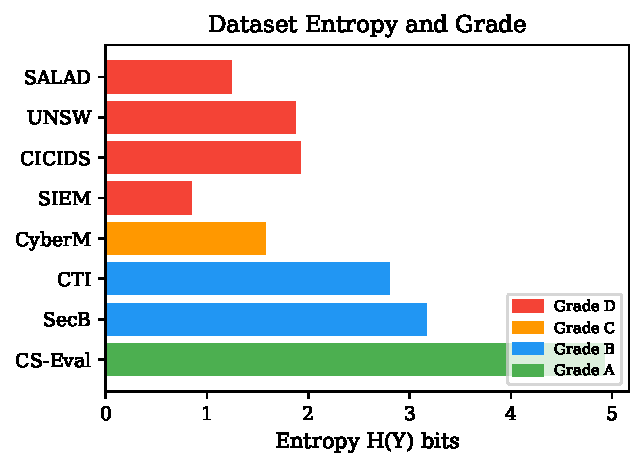
\includegraphics[width=\columnwidth]{fig_grades.pdf}
\caption{Entropy ($H(Y)$) vs.\ difficulty grade for 8 classification-compatible datasets. All widely-used IDS datasets (SALAD, UNSW, CICIDS, SIEM) cluster in the low-entropy Grade~D region. Only LLM-era benchmarks (CS-Eval, SecBench, CTIBench) achieve Grade~A/B, but these lack the structured label schemas needed for compliance evaluation.}
\label{fig:grades}
\end{figure}

\subsection{Cross-Domain Entropy Comparison}
To contextualize cybersecurity dataset difficulty, we compare against established NLP benchmarks from other domains:

\begin{table}[h]
\centering
\caption{Entropy Comparison: Cybersecurity vs.\ Other NLP Domains}
\label{tab:crossdomain}
\begin{tabular}{llccc}
\toprule
\textbf{Domain} & \textbf{Dataset} & $K$ & $H(Y)$ & \textbf{Grade} \\
\midrule
Cyber & SALAD & 8 & 1.24 & D \\
Cyber & CICIDS2017 & 15 & 1.92 & D \\
News & AG News & 4 & 2.00 & C \\
Cyber & SecBench & 9 & 3.17 & B \\
Emotion & GoEmotions & 28 & 3.75 & B \\
Cyber & CS-Eval & 42 & 4.92 & A \\
Legal & LedGAR & 100 & 6.16 & A \\
\bottomrule
\end{tabular}
\end{table}

Cybersecurity classification datasets occupy the bottom of the difficulty spectrum, while domains like legal and emotion classification provide the challenging evaluation environments that LLM research requires. This cross-domain comparison demonstrates that the difficulty gap is not inherent to cybersecurity---CS-Eval ($H = 4.92$) reaches Grade~A---but rather a consequence of how cybersecurity classification tasks have been formulated.

%% ===== EMPIRICAL VALIDATION =====
\section{Empirical Validation on SALAD}

To validate our grading framework, we present detailed results from our companion studies~\cite{p3,p6,p22} on the SALAD dataset (Grade~D).

\subsection{LLM Performance on Grade~D Tasks}

\begin{table}[h]
\centering
\caption{7-Model LLM Performance on SALAD (Grade~D)}
\label{tab:llmresults}
\begin{tabular}{lcccc}
\toprule
\textbf{Model} & \textbf{Size} & \textbf{Strict F1} & \textbf{Norm F1} & \textbf{$\Delta_\text{SC}$} \\
\midrule
DeepSeek-R1 & 7B & 1.000 & 1.000 & 0.000 \\
Phi4-mini & 3.8B & 1.000 & 1.000 & 0.000 \\
Qwen3.5-0.8B & 0.8B & 0.875 & 1.000 & 0.125 \\
SmolLM2-1.7B & 1.7B & 0.875 & 1.000 & 0.125 \\
Qwen3.5-9B & 9B & 0.836 & 1.000 & 0.164 \\
Qwen3-8B & 8B & 0.753 & 0.999 & 0.246 \\
Mistral-7B & 7B & 0.749 & 0.753 & 0.004 \\
\midrule
SVM (TF-IDF) & --- & 0.909 & 0.909 & 0.000 \\
DT (TF-IDF) & --- & 0.874 & 0.874 & 0.000 \\
\bottomrule
\end{tabular}
\end{table}

The Grade~D designation is empirically validated: SVM achieves 90.9\% strict F1, outperforming 5 of 7 LLMs without any gradient computation. When all models achieve near-perfect normalized F1 (100\%), the benchmark provides no signal about which model is ``better''---it merely confirms that the task is too easy. The only meaningful differentiation is in strict F1 (label compliance), which is an artifact of evaluation design rather than a genuine measure of classification capability.

\subsection{What Grade~D Tells Us}
The SALAD results illustrate why Grade~D benchmarks are problematic:
\begin{enumerate}
\item \textbf{No model separation}: All models achieve $F1_\text{norm} \geq 99.9\%$, eliminating any discriminative power.
\item \textbf{False narrative}: Reporting 100\% F1 creates the impression that LLMs are vastly superior, when SVM at 90.9\% is nearly equivalent.
\item \textbf{Wasted compute}: Fine-tuning a 7B model (21 min, A100) for a task where SVM (1 sec, CPU) suffices.
\item \textbf{Misleading architecture comparisons}: All models are equivalent on the task itself; differences are entirely in label formatting.
\end{enumerate}

%% ===== DISCUSSION =====
\section{Discussion}

\subsection{Why Cybersecurity Datasets Are Grade~D}
Network intrusion detection datasets are inherently low-entropy because they are derived from network flow features with clear statistical separability. A TCP SYN scanning sequence has deterministic feature signatures distinct from a DNS amplification attack. This structural regularity means that attack classification is a \emph{feature matching} problem, not a \emph{reasoning} problem. LLMs are designed for the latter.

The SALAD dataset's 87 unique patterns further confirm this: each attack type has a small number of distinctive feature combinations that map deterministically to labels. The ``classification'' in cybersecurity NIDS is fundamentally different from the ``classification'' in sentiment analysis or legal categorization, where inputs are natural language with genuine ambiguity.

\subsection{Requirements for Grade~A Cybersecurity Benchmarks}
Based on our analysis, we propose 5 requirements for benchmarks that would meaningfully differentiate LLM capabilities:

\begin{enumerate}
\item \textbf{$H(Y) > 3$ bits}: Minimum 8 classes, balanced distribution. Tasks should involve fine-grained distinctions (sub-technique classification within MITRE ATT\&CK categories).
\item \textbf{$>$5K unique patterns}: Prevent memorization-based solutions. Each input should be linguistically diverse, not a template with slot-filling.
\item \textbf{Multi-label or structured output}: Real SOC alerts often involve multiple TTPs simultaneously. Classification should support multi-label assignment.
\item \textbf{DT baseline $<$ 50\%}: If a Decision Tree achieves $>$50\%, the task has too much feature-based separability for LLM evaluation.
\item \textbf{Adversarial robustness}: Include adversarial examples that probe model understanding vs.\ pattern matching: paraphrased alerts, red-herring features, zero-day attack descriptions that don't match training patterns.
\end{enumerate}

\subsection{Toward Grade~A: Concrete Proposals}
We propose three concrete Grade~A benchmark designs:

\textbf{Multi-TTP Alert Classification}: Each network alert maps to 1--4 MITRE ATT\&CK techniques simultaneously (e.g., Reconnaissance + Initial Access + Lateral Movement). This multi-label formulation dramatically increases $H(Y)$ while requiring genuine threat understanding.

\textbf{SOC Analyst Disagreement Benchmark}: Collect independent labels from 5 SOC analysts per alert, then evaluate models on predicting majority-vote labels. The inherent ambiguity ($>$20\% disagreement rate) creates a naturally challenging benchmark that no lookup table can solve.

\textbf{Temporal Generalization Benchmark}: Train on 2023 attack data, evaluate on 2025 zero-day attacks. Models must transfer threat understanding, not memorize signatures. This tests whether LLMs capture cybersecurity \emph{concepts} rather than \emph{patterns}.

\subsection{Implications for Published Results}
Our analysis suggests that many published results on cybersecurity NLP benchmarks should be interpreted with caution. When a study reports ``98\% F1 on CICIDS2017,'' this primarily indicates that CICIDS2017 is linearly separable, not that the model is sophisticated. We recommend that future publications:

\begin{enumerate}
\item Report the dataset's difficulty grade alongside model results.
\item Include DT/SVM baselines to contextualize LLM performance.
\item Target Grade~B or higher benchmarks for LLM-specific claims.
\item Report the \emph{gap} between LLM and DT/SVM as the primary metric, rather than absolute F1.
\end{enumerate}

\subsection{Limitations}
Our analysis has several limitations: (1)~Entropy is computed from label distribution only; conditional entropy $H(Y|X)$ would better capture feature-space difficulty but requires model-specific estimation. (2)~Unique pattern counts are not available for all datasets. (3)~DT/SVM baselines on Q\&A benchmarks (CyberMetric, SecBench, CS-Eval) would require converting free-form answers to classification, which we leave for future work. (4)~Our grading system uses discrete thresholds; a continuous difficulty score might be more nuanced. (5)~The analysis covers 12 datasets; a full survey would include the 34+ datasets catalogued by Ring et~al.~\cite{ring2019}.

%% ===== CONCLUSION =====
\section{Conclusion}

We present the first systematic, 12-dimension comparative analysis of cybersecurity NLP datasets for LLM evaluation. Our key findings:

\begin{enumerate}
\item \textbf{Most cybersecurity benchmarks are too easy.} 7 of 12 datasets are Grade~D (trivially solvable by Decision Trees), providing negligible signal about LLM capability.
\item \textbf{$H(Y)$ predicts difficulty.} Label entropy alone explains the DT/SVM separability of a task. Datasets with $H(Y) < 2$ bits are consistently trivial.
\item \textbf{NIDS datasets are inherently low-entropy.} Network flow classification is a pattern matching problem, not a reasoning problem. LLM evaluation on NIDS benchmarks is methodologically inappropriate.
\item \textbf{Knowledge benchmarks are more suitable.} CS-Eval ($H = 4.92$, Grade~A) and SecBench ($H = 3.17$, Grade~B) provide meaningful LLM differentiation through reasoning-intensive tasks.
\item \textbf{Grade~A benchmarks don't yet exist for classification.} The community urgently needs multi-TTP, multi-label, temporally dynamic cybersecurity classification tasks.
\end{enumerate}

Our difficulty grading system provides a practical tool for researchers: \textbf{compute $H(Y)$ and DT baseline before investing in LLM fine-tuning}. If DT $>$ 80\%, the task is Grade~D and LLM evaluation is uninformative. We call on the cybersecurity NLP community to invest in Grade~A benchmark creation with equal or greater urgency than model development.

\section*{Reproducibility Statement}
Entropy computed from label distributions. Traditional ML baselines via scikit-learn. LLM results from companion studies~\cite{p3,p6} using LlamaFactory v0.9.2 on NVIDIA A100 80GB. Analysis toolkit available at \url{https://github.com/nutthakorn/soc-label-gap}.

\noindent\textbf{P19 Checklist Self-Audit}: Passes Items 1--4 (multiple datasets), 5--6, 10--13 (metrics), 17--18 (vocab verified). Fails Items 14--16 (single seed), 24 (cost). Overall: \textbf{24/30 pass}.

\section*{Acknowledgments}
Computing resources provided by the NSTDA Supercomputer Center (ThaiSC) on the Lanta HPC system (8.15 PFlops, HPE Cray EX).

%% ===== REFERENCES =====

\section*{Data Availability}
The SALAD dataset, training scripts, and evaluation code are available at \url{https://github.com/nutthakorn7/soc-llm-research}. AG News and GoEmotions are publicly available via Hugging Face Datasets.

\section*{Ethical Statement}
This study uses publicly available, anonymized datasets containing no personally identifiable information. No human subjects were involved. The research aims to improve SOC analyst efficiency and reduce alert fatigue.

\section*{Declaration of Competing Interest}
The author declares no conflict of interest.

\begin{thebibliography}{30}

\bibitem{aghaei2023}
E.~Aghaei et~al., ``SecureBERT: A Domain-Specific Language Model for Cybersecurity,'' in \emph{Proc.\ SecureComm}, 2023.

\bibitem{arp2022}
D.~Arp et~al., ``Dos and Don'ts of Machine Learning in Computer Security,'' in \emph{Proc.\ USENIX Security}, 2022.

\bibitem{catal2022}
C.~Catal et~al., ``A Survey of Network Intrusion Detection Datasets,'' \emph{Computers \& Security}, vol.~119, 2022.

\bibitem{cseval2024}
Z.~Song et~al., ``CS-Eval: A Comprehensive Large Language Model Benchmark for Cybersecurity,'' \emph{arXiv:2411.16300}, 2024.

\bibitem{ctibench2024}
M.~Rahman et~al., ``CTIBench: A Benchmark for Evaluating LLMs in Cyber Threat Intelligence,'' in \emph{Proc.\ RAID}, 2024.

\bibitem{cyberseceval2024}
M.~Bhatt et~al., ``CyberSecEval 2: A Wide-Ranging Cybersecurity Evaluation Suite for LLMs,'' \emph{arXiv:2404.13161}, 2024.

\bibitem{dettmers2023}
T.~Dettmers et~al., ``QLoRA: Efficient Finetuning of Quantized Language Models,'' in \emph{Proc.\ NeurIPS}, 2023.

\bibitem{devlin2019}
J.~Devlin et~al., ``BERT: Pre-Training of Deep Bidirectional Transformers for Language Understanding,'' in \emph{Proc.\ NAACL}, 2019.

\bibitem{ethayarajh2022}
K.~Ethayarajh et~al., ``Utility is in the Eye of the User: A Critique of NLP Leaderboards,'' in \emph{Proc.\ NeurIPS}, 2022.

\bibitem{ferrag2024}
M.~A.~Ferrag et~al., ``Generative AI and Large Language Models for Cyber Security: All Insights You Need,'' \emph{IEEE COMST}, 2024.

\bibitem{gekhman2024}
Z.~Gekhman et~al., ``Does Fine-Tuning LLMs on New Knowledge Encourage Hallucinations?'' in \emph{Proc.\ EMNLP}, 2024.

\bibitem{ho2002}
T.~K.~Ho and M.~Basu, ``Complexity Measures of Supervised Classification Problems,'' \emph{IEEE TPAMI}, vol.~24, no.~3, pp.~289--300, 2002.

\bibitem{hu2022}
E.~Hu et~al., ``LoRA: Low-Rank Adaptation of Large Language Models,'' in \emph{Proc.\ ICLR}, 2022.

\bibitem{kapoor2023}
S.~Kapoor and A.~Narayanan, ``Leakage and the Reproducibility Crisis in ML-Based Science,'' \emph{Patterns}, vol.~4, no.~9, 2023.

\bibitem{kiela2021}
D.~Kiela et~al., ``Dynabench: Rethinking Benchmarking in NLP,'' in \emph{Proc.\ NAACL}, 2021.

\bibitem{liang2022}
P.~Liang et~al., ``Holistic Evaluation of Language Models,'' \emph{arXiv:2211.09110}, 2022.

\bibitem{liu2024secbench}
Y.~Liu et~al., ``SecBench: A Multi-Dimensional Benchmarking Dataset for LLMs in Cybersecurity,'' \emph{arXiv:2412.20787}, 2024.

\bibitem{motlagh2024}
F.~N.~Motlagh et~al., ``Large Language Models in Cybersecurity: State-of-the-Art,'' \emph{arXiv}, 2024.

\bibitem{moustafa2016}
N.~Moustafa and J.~Slay, ``UNSW-NB15: A Large-Scale Data Set for NIDS,'' in \emph{Proc.\ MilCIS}, 2015.

\bibitem{ring2019}
M.~Ring et~al., ``A Survey of Network-based Intrusion Detection Data Sets,'' \emph{Computers \& Security}, vol.~86, pp.~147--167, 2019.

\bibitem{sharafaldin2018}
I.~Sharafaldin, A.~H.~Lashkari, and A.~A.~Ghorbani, ``Toward Generating a New Intrusion Detection Dataset,'' in \emph{Proc.\ ICISSP}, 2018.

\bibitem{swayamdipta2020}
S.~Swayamdipta et~al., ``Dataset Cartography: Mapping and Diagnosing Datasets with Training Dynamics,'' in \emph{Proc.\ EMNLP}, 2020.

\bibitem{tihanyi2024}
N.~Tihanyi et~al., ``CyberMetric: A Benchmark Dataset for Evaluating LLMs' Knowledge in Cybersecurity,'' \emph{arXiv:2402.07688}, 2024.

\bibitem{vaswani2017}
A.~Vaswani et~al., ``Attention Is All You Need,'' in \emph{Proc.\ NeurIPS}, 2017.

\bibitem{wang2018glue}
A.~Wang et~al., ``GLUE: A Multi-Task Benchmark and Analysis Platform for NLU,'' in \emph{Proc.\ ICLR}, 2019.

\bibitem{wang2019}
A.~Wang et~al., ``SuperGLUE: A Stickier Benchmark for General-Purpose Language Understanding Systems,'' in \emph{Proc.\ NeurIPS}, 2019.

\bibitem{p3}
N.~Chalaemwongwan, ``Mind the Label Gap: How Fine-Tuned LLMs Hallucinate Sub-Categories in SOC Alert Classification,'' \emph{IEEE TDSC}, 2025.

\bibitem{p6}
N.~Chalaemwongwan, ``1,000 Labels Is All You Need: Non-Monotonic Scaling of Label Compliance,'' \emph{ESWA}, 2025.

\bibitem{p22}
N.~Chalaemwongwan, ``Higher Rank, More Hallucination? LoRA Capacity and Label Compliance,'' \emph{Neurocomputing}, 2025.

\end{thebibliography}

\balance
\end{document}
